\section{Introduction}
\begin{frame}{Balloon Model}
\begin{figure}
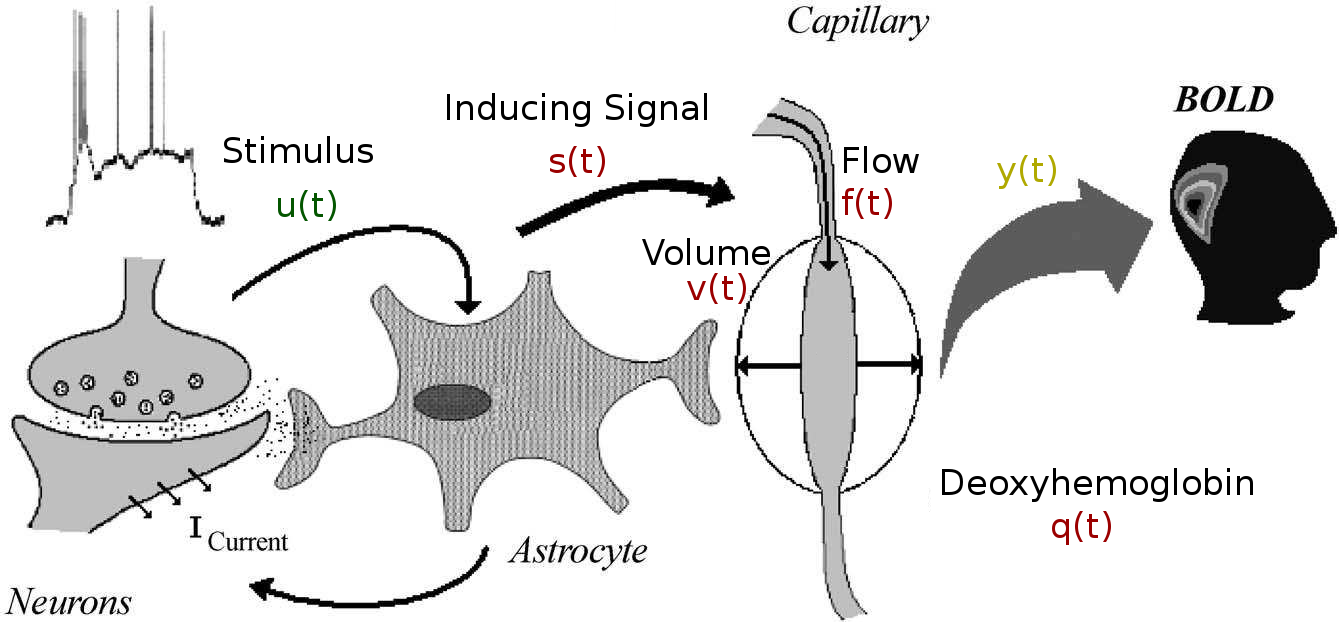
\includegraphics[width=10cm]{model2}
\caption{
    \tiny
    \cite{Riera2003}
}
\end{figure}
\note{
    \begin{itemize}
        \item FMRI has been around for about 20 years
        \item 10 Years Since the First BOLD Model
        \item Basis of FMRI, T2$^*$ relaxation time, blood oxygen levels
        \item Windkessel/Balloon Model, Volume Changes driving fluctations
            in blood oxygen 
        \item Brain has no local oxygen storage, dependent on blood
        \item brain active, firing rates of neurons increase 10 or 100x
        \item recharging requires additional oxygen ... metabolism. 
        \item Increased metabolism drives increased blood flow
        \item Increased blood flow increases volume
        
        \item Rates from below 1 Hz to 5 to 6 Hundred Hz
    \end{itemize}
}
\end{frame}

\begin{frame}{Activation Chain}
\begin{figure}
    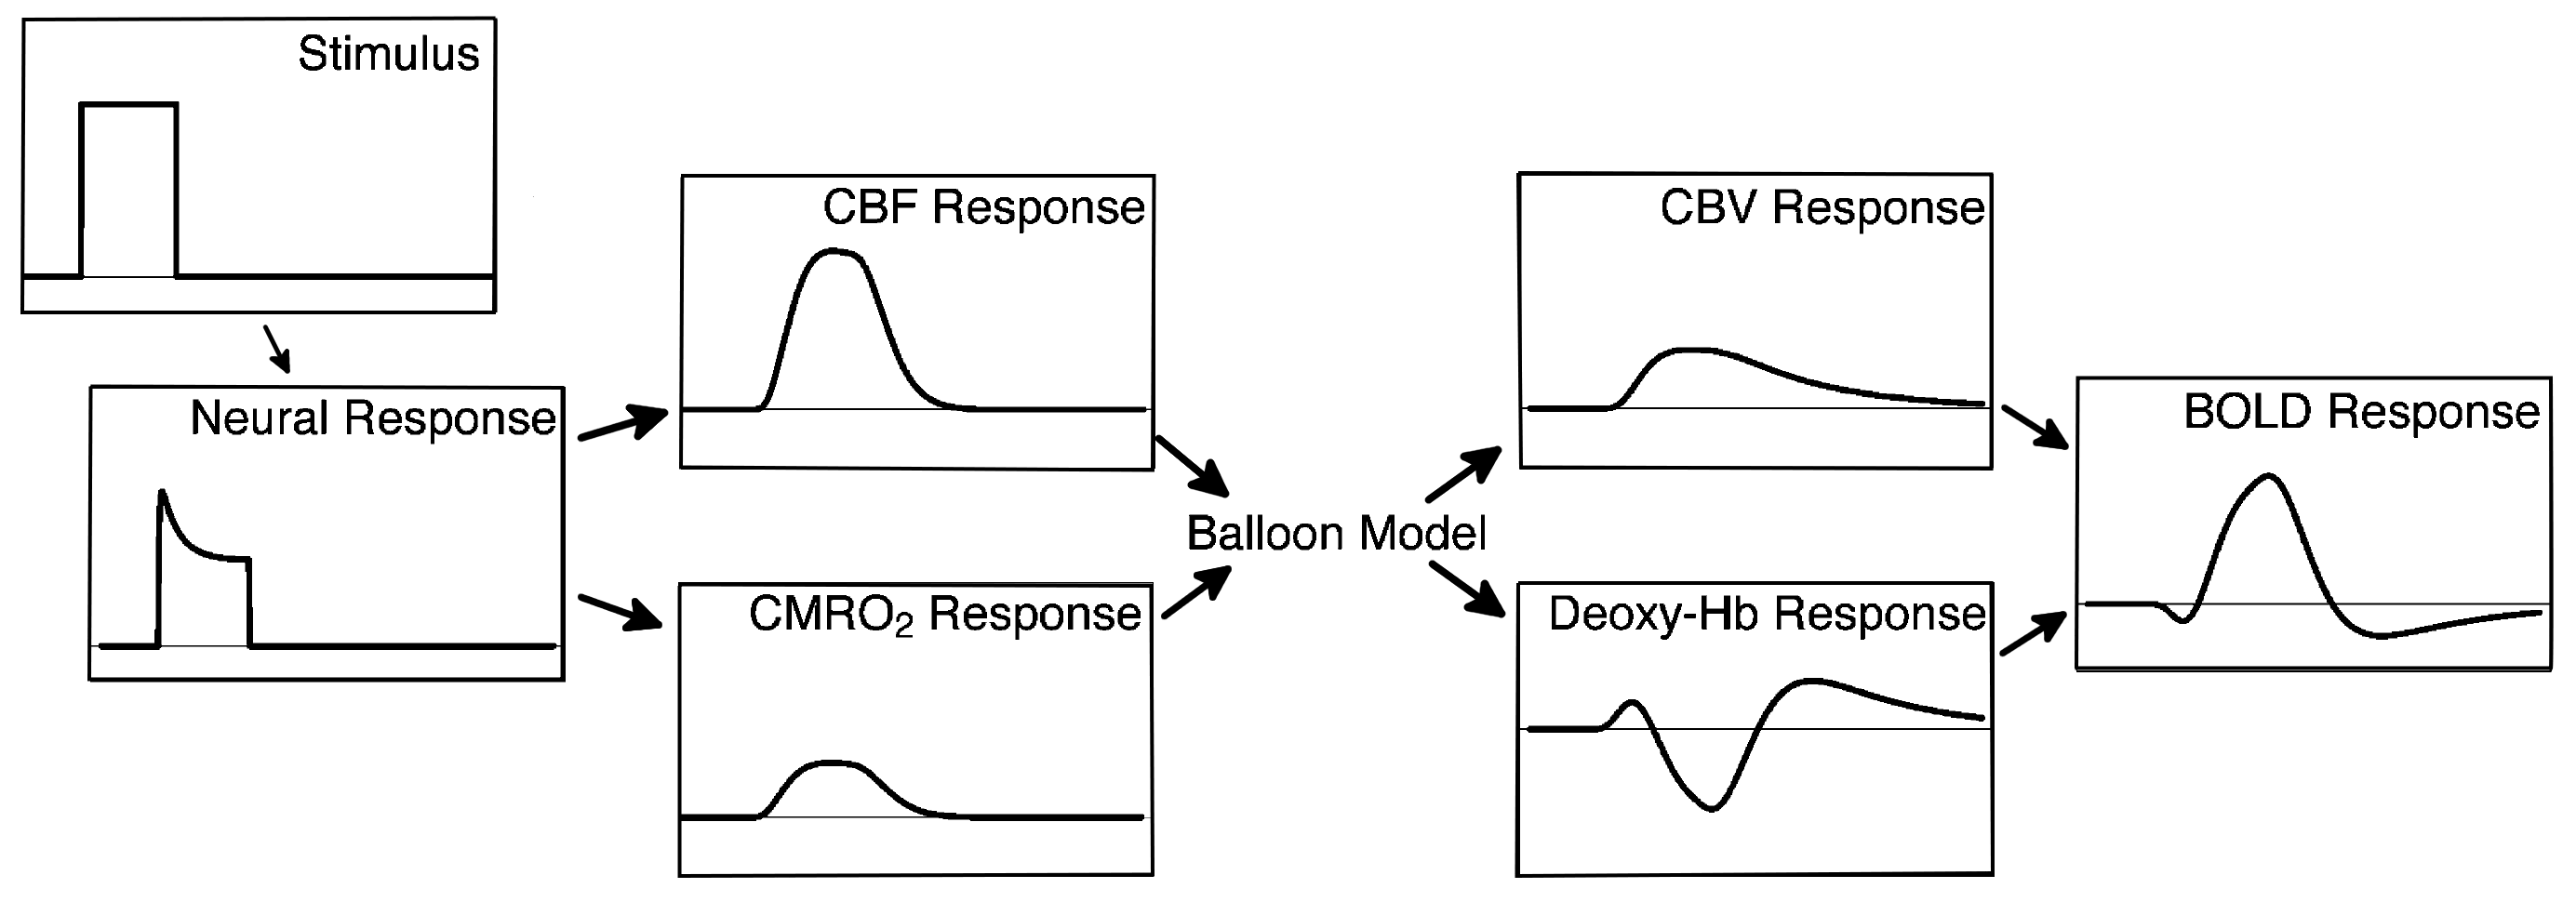
\includegraphics[width=\textwidth]{graphs}
\caption{
    \tiny
    \cite{Buxton2004}
}
\end{figure}
\note{
    \begin{itemize}
        \item CMRO2 Increased Metabolism Causes Initial Drop In Oxygen
        \item CBF Flow Quickly Compensates Increases Oxygen
        \item CBV Increases, Decides the outflow, local oxygen content
        \item This delays result in the characteristic BOLD response
        \item CBF CMRO2 Locked 
    \end{itemize}
}
\end{frame}

%more expansion of all the parameters
\begin{frame}{BOLD State Space Model}
  \scriptsize
  \begin{columns}
  \begin{column}{.7\textwidth}
    \begin{itemize}
    \item State Vector:
    \begin{eqnarray}
    \color{mblue}\dot{s}(t) &=& {\color{mred}\epsilon} {\color{mgreen}u(t)} - 
                \frac{\color{mblue}s(t)}{\color{mred}\tau_s} - \frac{{\color{mblue}f(t)}-1}{\color{mred}\tau_f} \nonumber \\
    \color{mblue}\dot{f}(t) &=& \color{mblue}s \nonumber \\
    \color{mblue}\dot{v}(t) &=& \frac{{\color{mblue}f(t)} - 
                {\color{mblue}v(t)} ^ {1/{\color{mred}\alpha}}}{\color{mred}\tau_0} \nonumber \\
    \color{mblue}\dot{q}(t) &=& \frac{1}{\color{mred}\tau_0}
            \left(\frac{{\color{mblue}f(t)}(1-(1-{\color{mred}E_0})^{1/\color{mblue}f(t)})}{\color{mred}E_0} -
        \frac{\color{mblue}q(t)}{{\color{mblue}v(t)}^{1-1/\color{mred}\alpha}}\right) \nonumber 
    \end{eqnarray}
    \item Output:
    $${\color{myellow}y(t)} = {\color{mred}V_0}(a_1( 1 - {\color{mblue}Q(t)}) - a_2(1 - {\color{mblue}V(t)}))$$
    \end{itemize}
  \end{column}

  \begin{column}{.3\textwidth}
    \begin{itemize}
        \item State Variables:
        $${\color{mblue}s(t)}, {\color{mblue}f(t)}, {\color{mblue}v(t)}, {\color{mblue}q(t)}$$
        \item Parameters:
        $${\color{mred}\epsilon}, {\color{mred}\tau_s}, {\color{mred}\tau_f}, {\color{mred}\alpha}, 
                    {\color{mred}\tau_0}, {\color{mred}E_0}, {\color{mred}V_0}$$
        \item Constants:
        $$a_1, a_2$$
        \item Input:
        $$\color{mgreen}u(t)$$
    \end{itemize}
  \end{column}
  \end{columns}
  \note{
    \tiny
    \begin{itemize}
    \item System is dissipative,
    \item Constant input leads to steady state 
    \item $u(t)$ is the input
    \item States
    \begin{itemize}
    \tiny
    \item s - Neural Response (Flow Inducing Signal)
    \item f - Inflow of Oxygenated Blood
    \item v - Local Blood Volume
    \item q - Deoxygenated hemoglobin content
    \end{itemize}
    \item Parameters
    \begin{itemize}
    \tiny
    \item $\epsilon$ - efficiency
    \item $\tau_s$ - Falloff time for Flow Inducing Signal
    \item $\tau_f$ - Onset time for Flow Inducing Signal
    \item $\alpha$ - Grubbs Constant determining outflow volume
    \item $\tau_0$ - Time Constant for volume, deoxygenated hemoglobin
    \item $E_0$ - Resting Oxygen Metabolism
    \item $V_0$ - Resting Metabolism
    \end{itemize}
    \item $a_1$,$a_2$ are functions of the imaging modality,
            and to a vary somewhat with $E_0$. 
    \item $a_1 = k_1*E_0 + k_2*E_0$, $a_2 = k_2*E_0 + k_3$
    \end{itemize}
  }
\end{frame}
